\documentclass[11pt,a4paper]{article}
\usepackage{graphicx}
\usepackage{geometry}
%\geometry{legalpaper, landscape, margin=2in} %to convert into slides
\usepackage[english]{babel}
\usepackage{pdfpages}
\usepackage{amsmath}
\usepackage{amsfonts}
\usepackage{bm} %Package for bold greek letters. Use for example $\bm{\Chi}$
\usepackage{eucal}
\usepackage{hyperref}
\hypersetup{
 colorlinks,
 citecolor = black,
 filecolor = black,
 linkcolor = black,
 urlcolor = black
}

\begin{document}

\title{Three points correlators}
\author{Kaons oscillations like}
\date{Emanuele Rosi, October 2023}
\maketitle

\begin{center}
    {\bf Abstract}\\
    Calculation of flavour non-singlet meson oscillations through the insertion \\ of intermediate operators and stochastic sources in QCD with open boundary conditions.
\end{center}

\section{Wick Contractions}
We want to calculate three points correlators of this two types:
\begin{equation}
    \begin{gathered}
        G_d(x_0,y_0,z_0) = \sum_{\vec x, \vec y, \vec z} \bigg\langle
        \bar\psi_4(x) \Gamma_A \psi_1 (x)\hspace*{.3mm}
        \bar\psi_3(y) \Gamma_D \psi_2 (y) \bar\psi_1(y) \Gamma_B \psi_4 (y)\hspace*{.3mm}
        \bar\psi_2(z) \Gamma_C \psi_3 (z)\hspace*{.3mm}
        \bigg\rangle^{\text{sea}}\\
        G_c(x_0,y_0,z_0) = \sum_{\vec x, \vec y, \vec z} \bigg\langle
        \bar\psi_4(x) \Gamma_A \psi_1 (x)\hspace*{.3mm}
        \bar\psi_3(y) \Gamma_D \psi_4 (y) \bar\psi_1(y) \Gamma_B \psi_2 (y)\hspace*{.3mm}
        \bar\psi_2(z) \Gamma_C \psi_3 (z)\hspace*{.3mm}
        \bigg\rangle^{\text{sea}}\\
    \end{gathered}
\end{equation}
the subscripts $c$ and $d$ refer to {\it connected} and {\it disconnected} correlators.
Picture \ref{figura_fig} shows the correlators in a simple representative way for $x_0>y_0>z_0$.
The Wick contractions acting on the correlators are:
\begin{equation}\label{eq:contractions}
    \begin{gathered}
        G_d(x_0,y_0,z_0) = \sum_{\vec x, \vec y, \vec z} \bigg\langle \text{Tr}\left[\Gamma_A S_1(x,y)\Gamma_B S_4(y,x)\right]\cdot\text{Tr}\left[\Gamma_C S_3(z,y)\Gamma_D S_2(y,z)\right] \bigg\rangle^{\text{sea}} \\
        G_c(x_0,y_0,z_0) = - \sum_{\vec x, \vec y, \vec z} \bigg\langle \text{Tr}\left[\Gamma_A S_1(x,y)\Gamma_B S_2(y,z)\Gamma_C S_3(z,y)\Gamma_D S_4(y,x)\right] \bigg\rangle^{\text{sea}}
    \end{gathered}
\end{equation}
\begin{figure}[h!]
    \centering
    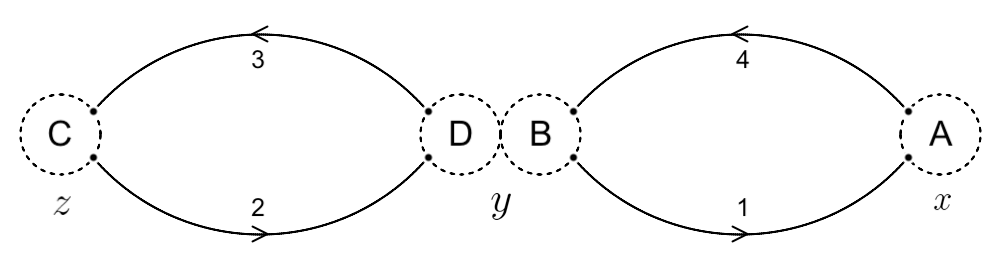
\includegraphics[width=0.9\textwidth]{include-imgs/Wick_disconnected.png}
    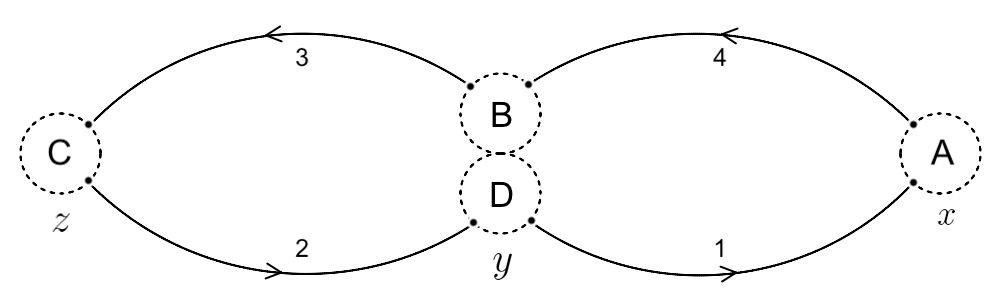
\includegraphics[width=0.8\textwidth]{include-imgs/Wick_connected.png}
    \caption{On the top: graph of disconnected Wick contraction. On the bottom: graph of connected Wick contraction.}
\end{figure}\label{figura_fig}
\newline
%There exists a simple way to evaluate these correlators.
%The method is based on the sheet by Tomasz Korzec for Meson correlators (2013) and it involves the use of stochastic spinors.
I generate $N_{\text{noise}}$ stochastic spinors in the timeslice $x_0$ and $N_{\text{noise}}$ stochastic spinors in the timeslice $z_0$.
I refer to the formers with $\eta^{1}$ and the latters with $\eta^{2}$.
These stochastic spinors have again a Dirac index ($\alpha,\beta,\cdots$) and a colour index ($a,b,\cdots$).
The properties \ref{eq:eta-properties} are generalized:
\begin{equation}
    \begin{gathered}
        \langle \eta^{1}_{a\alpha} (u) \rangle^{\text{noise}} = \langle \eta^{2}_{b\beta} (u) \rangle^{\text{noise}} = 0 \\
        \langle \eta^{1*}_{a\alpha} (u) \eta^{1}_{b\beta} (v) \rangle^{\text{noise}} = \delta_{a,b} \delta_{\alpha,\beta} \delta_{\vec u, \vec v} \delta_{u_0,x_0} \delta_{v_0,x_0} \\
        \langle \eta^{2*}_{a\alpha} (u) \eta^{2}_{b\beta} (v) \rangle^{\text{noise}} = \delta_{a,b} \delta_{\alpha,\beta} \delta_{\vec u, \vec v} \delta_{u_0,z_0} \delta_{v_0,z_0} \\
    \end{gathered}
\end{equation}
where the symbol $\langle\hspace{1mm}\cdot\hspace{1mm}\rangle^\text{noise}$ refers to the average over $N_{\text{noise}}$ vectors and $u,v \in \Lambda$ are lattice points.
I define derived stochastic vectors:
\begin{equation}
    \begin{aligned}
        & \zeta^{(i,\pm)}_{j} (u) = \sum_{v} S_{(i,\pm)}(u,v)\eta^{j}(v) \\
        & \xi^{(i,\pm)}_{j,X} (u) = \sum_{v} S_{(i,\pm)}(u,v) \gamma_5 \Gamma_X^\dag \eta^{j}(v)
    \end{aligned}
\end{equation}
A brief discussion about their indices could clarify the notation:
\begin{itemize}
    \item   $j=1,2$ is the stochastic vector index. It tells you whenever to use $\eta^{(1)}$ or $\eta^{(2)}$.
    \item   $X=A,B,C,D$ is the matrix index. It tells you to use $\Gamma_X^\dag \in \{\Gamma_A^\dag,\Gamma_B^\dag,\Gamma_C^\dag,\Gamma_D^\dag\}$.
    \item   $i=1,2,3,4$ refers to the propagator index. In principle, the $\psi_i$ s could be four different quarks.
    \item   the sign $\pm$ is referred to the twisted mass parameter. If you use maximally twisted mass QCD - or maximally twisted Osterwalder-Seiler regularization - you should remember that the propagator is obtained by the inversion:
               $$\sum_{w} \left(D_W^{(i)} \pm i\gamma_5\mu^{(i)}\right)(u,w) S_{(i,\pm)}(w,v) = \delta_{u,v}$$ 
            and I will use the following property: $\gamma_5 S_{(i,\pm)}^\dag(u,v) \gamma_5 = S_{(i,\mp)}(v,u)$ that explain the need of $\pm$ symbol.
    \item   the symbols $i$ and $\pm$ are referred to the same propagator. For this reason they are coupled as $(i,\pm)$.
\end{itemize}
It could be easily checked that the contractions in (\ref{eq:contractions}) can be obtained by the following formulae:
\begin{equation*}
    \begin{gathered}
        G_d(x_0,y_0,z_0) =   \sum_{\vec y} \left\langle \left\langle \left(\gamma_5\xi^{(1,-)}_{1,A} (y) \right)^\dag \Gamma_B \zeta^{(4,+)}_1 (y) \cdot \left(\gamma_5\xi^{(3,-)}_{C,2} (y) \right)^\dag \Gamma_D \zeta^{(2,+)}_2 (y) \right\rangle^\text{noise} \right\rangle^{\text{sea}} \\
        G_c(x_0,y_0,z_0) = - \sum_{\vec y} \left\langle \left\langle \left(\gamma_5\xi^{(1,-)}_{1,A} (y) \right)^\dag \Gamma_B \zeta^{(2,+)}_2 (y) \cdot \left(\gamma_5\xi^{(3,-)}_{C,2} (y) \right)^\dag \Gamma_D \zeta^{(4,+)}_1 (y) \right\rangle^\text{noise} \right\rangle^{\text{sea}}
    \end{gathered}
\end{equation*}
Then, to evaluate the previous couple of Wick contraction {\bf I need only four quantites} for each couple of stochastic spinors:
\begin{equation*}
    \xi^{(1,-)}_{1,A} (y) \qquad  \zeta^{(4,+)}_1 (y) \qquad \xi^{(3,-)}_{C,2} (y) \qquad  \zeta^{(2,+)}_2 (y)
\end{equation*}
The path to evaluate the correlators is:
\begin{itemize}
    \item [$\triangleright$] For each Gauge-sea configuration evaluate 2$N_{\text{noise}}$ spinors - $N_{\text{noise}}$ for $\eta^1$ and $N_{\text{noise}}$ for $\eta^2$. 
    \item [$\triangleright$] For each noise spinor evaluate the quantites $\zeta$ and $\xi$ needed. Sometimes just a few number of them are needed.
    \item [$\triangleright$] Evaluate the correlators and evaluate the noise average.
    \item [$\triangleright$] Iterate the procedure and calculate the sea average.
\end{itemize}



\end{document}